%%%%%%%%%%%%%%%%%%%%%%%%%%%%%%%%%%%%%%%%%%%%%%%%%%%%%
\chapter{Formulation as an Optimal Transport Problem}
The Damped Newton algorithm developed by M\'{e}rigot et al. \cite{Merigot2017} solves a semi-discrete Monge-Amp\`{e}re type optimal transport problem. It's efficiency in exploiting the properties of sparse matrices and linear convergence \cite{Merigot2017} make it practical for implementation in the solution for equations \ref{EadyGC}. Further detail describing the application of the algorithm in the solution to the Eady Model is given in chapter \ref{algorithm}. In this chapter an overview of semi-discrete optimal transport is given using definitions given in \cite{Kitagawa2016, Merigot2017} as well as a comparison to the energy minimisation to which it is applied. A rigorous proof of the formulation of \ref{EadyModel} as a Monge-Amp\`{e}re type optimal transport problem is given in Cullen, 2006 \cite{Cullen2006a}.
\section{Semi-discrete Optimal Transport}
\begin{figure}[h]
	\centering
	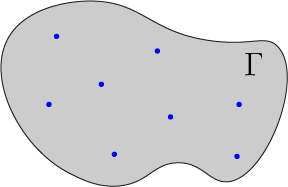
\includegraphics[width=5.5cm]{project/probmeasure}
	\caption[Semi-discrete Optimal Transport]{A discrete (target) set $Y \subseteq \mathbb{R}^2$ represented by blue points in a compact domain (source) $\Gamma \subseteq \mathbb{R}^2 $}
	\label{fig:probmeasure}
\end{figure}
Optimal transport problems describe the problem of finding a map between two sets, each with an associated density, in such a way that the "cost" associated with the mapping is minimised. In semi-discrete optimal transport the target set is a finite set.\\
\linebreak
In Kitagawa et al. \cite{Kitagawa2016} a wonderful analogy with travel distance to bakeries in a city is made. The example considers a population in the city and a finite set of locations of bakeries in the city. It is assumed that the population is uniformly distributed in the city. The optimal transport problem finds a partition of the city such that every point in a region of the partion is closest to the bakery at the centre of that region. In this analogy the cost being minimised is the travel distance to the bakery $c(\bm{x},\bm{y}_i) = \|\bm{x}-\bm{y}_i \|^2$. This is illustrated in figure \ref{fig:laguerrediagram0w}  below
\begin{figure}[h]
	\centering
	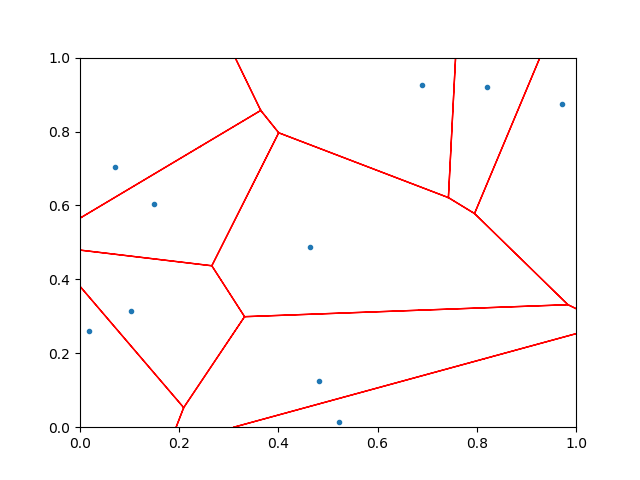
\includegraphics[width=7cm]{project/laguerre_diagram_0w}
	\caption[The partitioning of a city]{The image showing how a city would be divided into areas based on minimising distance to the local bakeries denoted by blue points}
	\label{fig:laguerrediagram0w}
\end{figure}
\\
To put this into a more rigorous mathematical setting, given a domain  $\Gamma\subseteq \mathbb{R}^2$ and discrete set of $N$ points $Y = \left\lbrace \bm{y}_i, \quad 1\leq i \leq N \right\rbrace  \subset \mathbb{R}^2$,\\
\linebreak
\textbf{Source measure} $\mu(A) = \int_A \rho(x)dx$, $A \subseteq \Gamma$ with $\rho$ a probability density on $\Gamma$\\
The \textbf{Target measure} $\nu = \sum_{1\leq i \leq N}\nu_i \delta_{y_i}$, with finite support on $\mathbb{R}^2$, where $\nu_i \in \mathbb{R}$ and $\delta_{y_i}$ is the delta function centred at the point $\bm{y}_i$\\
\linebreak
The partition of the city is described mathematically by \textbf{Voronoi Cells} \\ $\text{Vor}_y := \left\lbrace x \in \Gamma \; \text{st} \; \forall z \in Y \; c(x,y) \leq c(x,z) \right\rbrace$\\
\linebreak
Following \cite{Kitagawa2016} we then define a \textbf{Transport map}, $T: \Gamma \rightarrow Y$ between the source measure $\mu$ and the target measure on $Y$, $\mu$ if $T_{\#}\mu = \nu$.\\
\linebreak
The \textbf{Pushforward} of a measure $\mu$ by a map $T: \Gamma \rightarrow Y$ is $T_{\#}\mu = \sum_{\bm{y}_i \in Y} \mu \left( T^{-1}(\bm{y}_i) \right) \delta_{\bm{y}_i}$, the sum of the measures of the set mapped to the point $\bm{y}_i$ under $T$
\\
From these definitions we can see that the optimal transport map is given by,
\begin{equation}
	T(x) = \arg\min_{y\in Y}\left(c(x,y)\right)
\end{equation}
or equivalently if 
\begin{equation}
\nu_i = \mu\left(\text{Vor}_{y_i}\right)
\end{equation}
Figure \ref{fig:laguerrediagram0w} above shows the Voronoi diagram for the example of bakeries in a city
\comments{not sure about this section - also a lot of it is paraphrased from the \cite{Kitagawa2016} paper}
\subsection{Laguerre Cells and the Inclusion of weights}
 \begin{figure}[h]
	\centering
	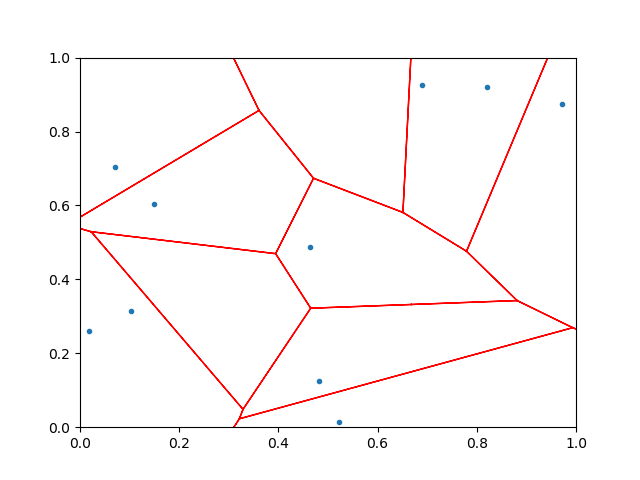
\includegraphics[width=7cm]{project/laguerre_diagram_OTw}
	\caption[Laguerre diagram produced by finding weights using damped newton algorithm for optimal transport]{Given a uniform source and target density the Laguerre diagram produced by finding weights using damped newton algorithm for optimal transport}
	\label{fig:laguerrediagramotw}
\end{figure}
Considering again the example of bakeries in the city, looking at figure \ref{fig:laguerrediagram0w} it is clear that if the population density across city is uniform the distribution of customers to each bakery is certainly not. For example, the Voronoi cell at the centre of the diagram is much larger in area than those in the top right of the diagram. This raises the problem of finding a way to create a partion so that each cell has the same area. This is done by introducing an additional \textquotedblleft weight \textquotedblright  argument to the cost. We denote the weights by $\psi_i = \psi\left(\bm{y}_i\right)$. In the case of the bakeries the weights might represent the price of bread at a specific bakery. For example in figure \ref{fig:laguerrediagram0w} if the bakery at the centre charged more for bread the population living on the outskirts of the cell would be more incentivised to travel further for cheaper bread.\\
\linebreak
The cells are now called  \textbf{Laguerre Cells}, defined as \\ $\text{Lag}_y(\psi) := \left\lbrace x \in K \; \text{st} \; \forall z \in Y \; c(x,y) + \psi(y) \leq c(x,z) + \psi(z) \right\rbrace$ \\ and the optimal transport map is given by \\
$T_\psi: x \rightarrow \text{argmin}_i\| x - y_i \|^2 + \psi_i$, where $\psi_i = \psi(y_i)$ is a family of weights on $Y$ \cite{Merigot2017}.\\
\linebreak
 The problem is then finding the weights $\psi_i$ associated to the points $y_i$ such that $G_i(\psi) := \mu (\text{Lag}_{y_i}(\psi)) = \nu_i$. The Damped Newton's Algorithm from M\'{e}rigot, Meyron and Thibert (2017) \cite{Merigot2017} finds such $\psi_i$.
 \\
 \linebreak 
 Supposing that both the source density and target density are uniform, the Laguerre cells as found by the code developed in \cite{Merigot2017} are show in figure \ref{fig:laguerrediagramotw}
\subsection{Applying semi-discrete optimal transport to solving the semi-geostrophic equations}
\section{Extension for Periodic Boundary Conditions}

%%%%%%%%%%%%%%%%%%%%%%%%%%%%%%%%%%%%%%%%%%%%%%%%%%%%%
\chapter{A Numerical Solution to the Eady Model for Frontogenesis \label{algorithm}}
\section{Initialisation of Points}
\section{Choice of initial weights}
\section{Time Stepping}
%%%%%%%%%%%%%%%%%%%%%%%%%%%%%%%%%%%%%%%%%%%%%%%%%%%%%
\chapter{Unsorted}
\section{Linear Stability Analysis}
Starting from the Eady Model \ref{EadyModel} restated below
\begin{equation}
	\begin{aligned}
	-fv_g + \frac{\partial \varphi}{\partial x} = 0,\\
	\frac{Dv_g}{Dt} + fu -\frac{Cg}{\theta _0}\left(z-H/2\right) = 0,\\
	\frac{D\theta'}{Dt} - Cv_g = 0,\\
	\frac{\partial \varphi}{\partial z} - g\frac{\theta'}{\theta_0} = 0,\\
	\nabla \cdot \bm{u} = 0.
	\end{aligned}
\label{EadyModel2}
\end{equation} 
Linearise about a base state given by Hoskins \cite{Hoskins1975},
\begin{equation}
	\begin{aligned}
		\bar{\theta} &= \theta_0 \frac{N_0^2\theta_0 z}{g} - Cy \\
		\bar{\varphi} &= \theta_0 + \frac{N_0^2 z^2}{2}\\
		\bar{v}_g &= 0\\
		\bar{U} &= \frac{Cg}{f\theta_0}\left(z - H/2\right)\\
		\bar{W} &= 0 
	\end{aligned}
\end{equation}
Introduce a perturbation and linearise about base state,\\
$u = \bar{U} + u'$, $w = w'$, $v_g =  v_g'$, $\varphi = \bar{\varphi} + \varphi'$, $\theta ' = \bar{\theta} + \theta ''$\\
Introducing the stream function,
\begin{equation}
	u' = \frac{\partial \psi}{\partial z},\qquad w' = -\frac{\partial \psi}{\partial x} 
\end{equation}
Looking for normal modes solutions of the form,
\begin{equation}
q' = \hat{q}(z)\exp^{i \left(kx - \omega t\right)}
\end{equation}
Equations \ref{EadyModel2} become,
\begin{align}
 		-f\hat{v}_g + ik\hat{\varphi} = 0,\label{stab1}\\
 	-i\omega \hat{v}_g + ik\bar{U}\hat{v}_g + f\frac{\text{d}\hat{\psi}}{\text{d}z} = 0,\label{stab2}\\
 	-i \omega \hat{\theta} + i k \bar{U} \hat{\theta} - ik\frac{N_0^2\theta_0}{g} \hat{\psi} - C\hat{v}_g = 0,\label{stab3}\\
 	\frac{\text{d}\hat{\varphi}}{\text{d}z} - g\frac{\hat{\theta}}{\theta_0} = 0 \label{stab4},
\end{align}
First eliminating, $\varphi$, equations \ref{stab1} and \ref{stab4} give,
\begin{equation}
	-f\frac{\text{d}\hat{v}_g}{\text{d}z}+ik\frac{\text{d}\hat{\varphi}}{\text{d}z} = 0, \qquad \frac{\text{d}\hat{\varphi}}{\text{d}z} - g\frac{\hat{\theta}}{\theta_0} = 0
\end{equation}
so that,
\begin{equation}
	\hat{\theta} = \frac{f\theta_0}{ikg} \frac{\text{d}\hat{v}_g}{\text{d}z}
\label{thetahat}
\end{equation}
Rearranging equation \ref{stab3}
\begin{equation}
	 i\left( k \bar{U} - \omega \right) \hat{\theta} - ik\frac{N_0^2\theta_0}{g} \hat{\psi} - C\hat{v}_g = 0
\label{stab3.1}
\end{equation}
eliminate $\hat{\theta}$ using \ref{thetahat}
\begin{equation}
	\frac{f\theta_0}{kg}\left( k \bar{U} - \omega \right)  \frac{\text{d}\hat{v}_g}{\text{d}z} - ik\frac{N_0^2\theta_0}{g} \hat{\psi} - C\hat{v}_g = 0
\label{vg}
\end{equation}
from equation \ref{stab2} we have
\begin{equation}
i\left( k \bar{U} - \omega \right) \hat{v}_g - f \frac{\text{d}\hat{\psi}}{\text{d}z} = 0
\label{stab2.1}
\end{equation}
differentiating this expression we find
\begin{equation*}
	ik \frac{\text{d}\bar{U}}{\text{d}z} \hat{v}_g + i(k\bar{U}-\omega)\frac{\text{d}\hat{v}_g}{\text{d}z} + f\frac{\text{d}^2{\psi}}{\text{d}z^2} = 0 
\end{equation*}
Substituting this expression with \ref{stab2.1} into \ref{stab3.1}, noting that,
\begin{equation*}
	(k\bar{U}-\omega)\frac{\text{d}\hat{v}_g}{\text{d}z} = if\frac{\text{d}^2{\psi}}{\text{d}z^2} + \frac{fk}{i(k\bar{U}-\omega)}\frac{\text{d}\bar{U}}{\text{d}z}\frac{\text{d}\hat{\psi}}{\text{d}z}
\end{equation*}
\begin{equation*}
	\frac{f\theta_0}{kg}\left(if\frac{\text{d}^2{\psi}}{\text{d}z^2} + \frac{fk}{i(k\bar{U}-\omega)}\frac{\text{d}\bar{U}}{\text{d}z}\frac{\text{d}\hat{\psi}}{\text{d}z}\right) - \frac{ik N_0^2\theta_0\hat{\psi}}{g} + \frac{Cf}{i(k\bar{U}-\omega)}\frac{\text{d}\psi}{\text{d}z} =0
\end{equation*}
Rearranging gives,
\begin{equation}
	-\frac{f^2\theta_0}{kg}(k\bar{U}-\omega)\frac{\text{d}^2{\psi}}{\text{d}z^2}+\left(Cf+\frac{f^2\theta_0}{g}\frac{\text{d}\bar{U}}{\text{d}z}\right)\frac{\text{d}\hat{\psi}}{\text{d}z}+\frac{ik N_0^2\theta_0}{g}(k\bar{U}-\omega)\hat{\psi}=0
\end{equation}
\begin{equation}
-\frac{f^2\theta_0}{kg}(k\bar{U}-\omega)\frac{\text{d}^2{\psi}}{\text{d}z^2}+2Cf\frac{\text{d}\hat{\psi}}{\text{d}z}+\frac{k N_0^2\theta_0}{g}(k\bar{U}-\omega)\hat{\psi}=0
\end{equation}
We reformulate this as a matrix eigenvalue problem for $\omega$
\begin{equation}
-f^2\theta_0\bar{U}\frac{\text{d}^2{\psi}}{\text{d}z^2}+2Cfg\frac{\text{d}\hat{\psi}}{\text{d}z}+k^2 N_0^2\theta_0k^2\bar{U}\hat{\psi}=\omega \left(kN_0^2\theta_0\hat{\psi}-\frac{f^2\theta_0 g}{k}\frac{\text{d}^2{\psi}}{\text{d}z^2}\right)
\end{equation}
Introducing a second order finite difference scheme for $\psi$
\begin{equation}
	\begin{aligned}
	\frac{\text{d}^2{\psi}}{\text{d}z^2} = \frac{\psi_{i-1} - \psi_i + \psi_{i+1}}{h^2}
	\frac{\text{d}\hat{\psi}}{\text{d}z} = \frac{\psi{i-1} - \psi_{i+1}}{2h}
	\end{aligned}
\end{equation}